\section{Implementação}

Pode-se dividir a implementação em seis partes, sendo elas: segmentar imagens, selecionar contorno, gerar proceduralmente o mapa com biomas, criar testes para avaliar a geração procedural, analisar casos de pós processamento e interligar as ferramentas através de uma interface gráfica.

\subsection{Segmentar imagens}

A segmentação da imagem é usada para classificar os píxeis da imagem a partir de padrões reconhecidos por uma inteligência artificial. A partir disso é possível o usuário selecionar o contorno para gerar o mapa \cite{dp_semantic_segmantation, lapix}.

Para a fotografia urbana, utilizou-se o modelo EfficientPS que segundo \citeonline{mohan2020efficientps} é uma solução eficiente para a segmentação panóptica. E também o código postado no repositório de \citeonline{efficientpsGit}.

Utilizou-se um arquivo pré treinado desse modelo contendo o aprendizado do conjunto de imagens do \textit{Cityscapes} para segmentação panóptica, a ideia inicial era treinar com pelo menos mais um conjunto de dados porém surgiu-se diversos desafios para serem solucionados, dentre eles: conseguir autorização para baixar conjuntos de dados específicos para segmentação panóptica, outro problema foi preparar esse conjunto de dados para processar o aprendizado, além de problemas de limitação de processamento bruto. Portante decidiu-se utilizar o próprio modelo salvo baixado do repositório.

Percebeu-se que o resultado do modelo proposto não foi o esperado pois objetos de mesma classe como carros tem a mesma cor com uma borda branca exemplificados na \cref{fig:resultado_inicial}. Logo tentou-se mudar o código para gerar uma saída com objetos de mesma classe com cores diferentes como na figura \cref{fig:expectativa} que está no artigo do EfficientPS por \citeonline{mohan2020efficientps}, no qual cada objeto da classe carro tem uma cor diferente e não tem borda entre os objetos.

\begin{figure}[!ht]
	\centering
    \caption{Resultado inicial do EfficientPS.}
	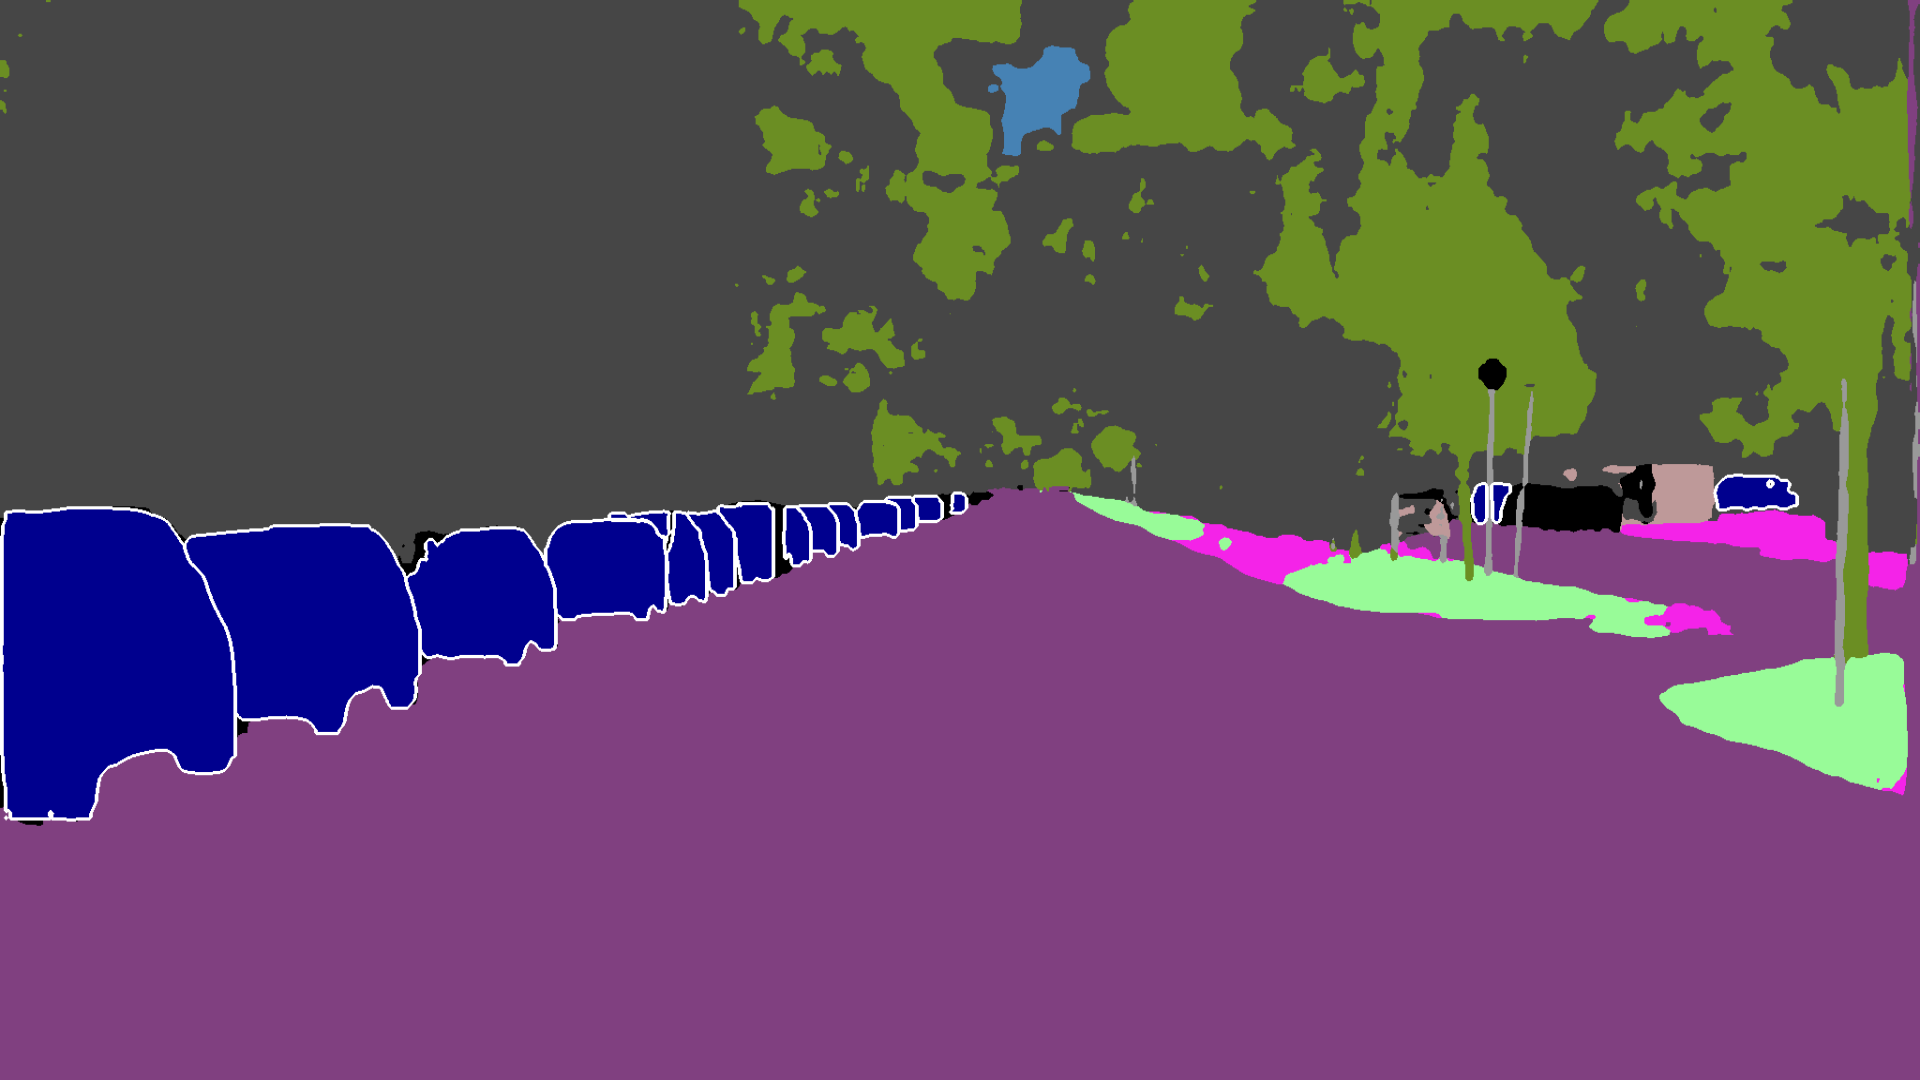
\includegraphics[width=0.6\textwidth]{figures/resultado_primario.png}
    \legend{Fonte: Criação própria}
	\label{fig:resultado_inicial}
\end{figure}

\begin{figure}[!ht]
	\centering
    \caption{Expectativa do resultado do EfficientPS.}
	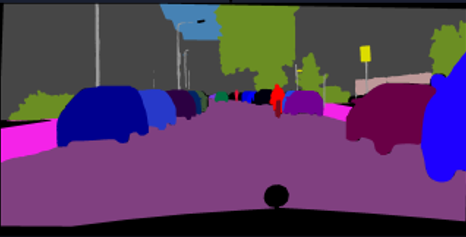
\includegraphics[width=0.6\textwidth]{figures/expectativa.png}
    \legend{Fonte: \citeonline{mohan2020efficientps}}
	\label{fig:expectativa}
\end{figure}

Seguiu-se os passos citados em uma publicação de \citeonline{efficientps_issue23} no repositório de \citeonline{efficientpsGit} porém o resultado obtido não foi satisfatório pois não foi possível discernir quais segmentos pertenciam as respectivas classes, o resultado é ilustrado na \cref{fig:resultado_obtido}.

\begin{figure}[!ht]
	\centering
    \caption{Resultado do EfficientPS obtido seguindo os passos da publicação no repositório.}
	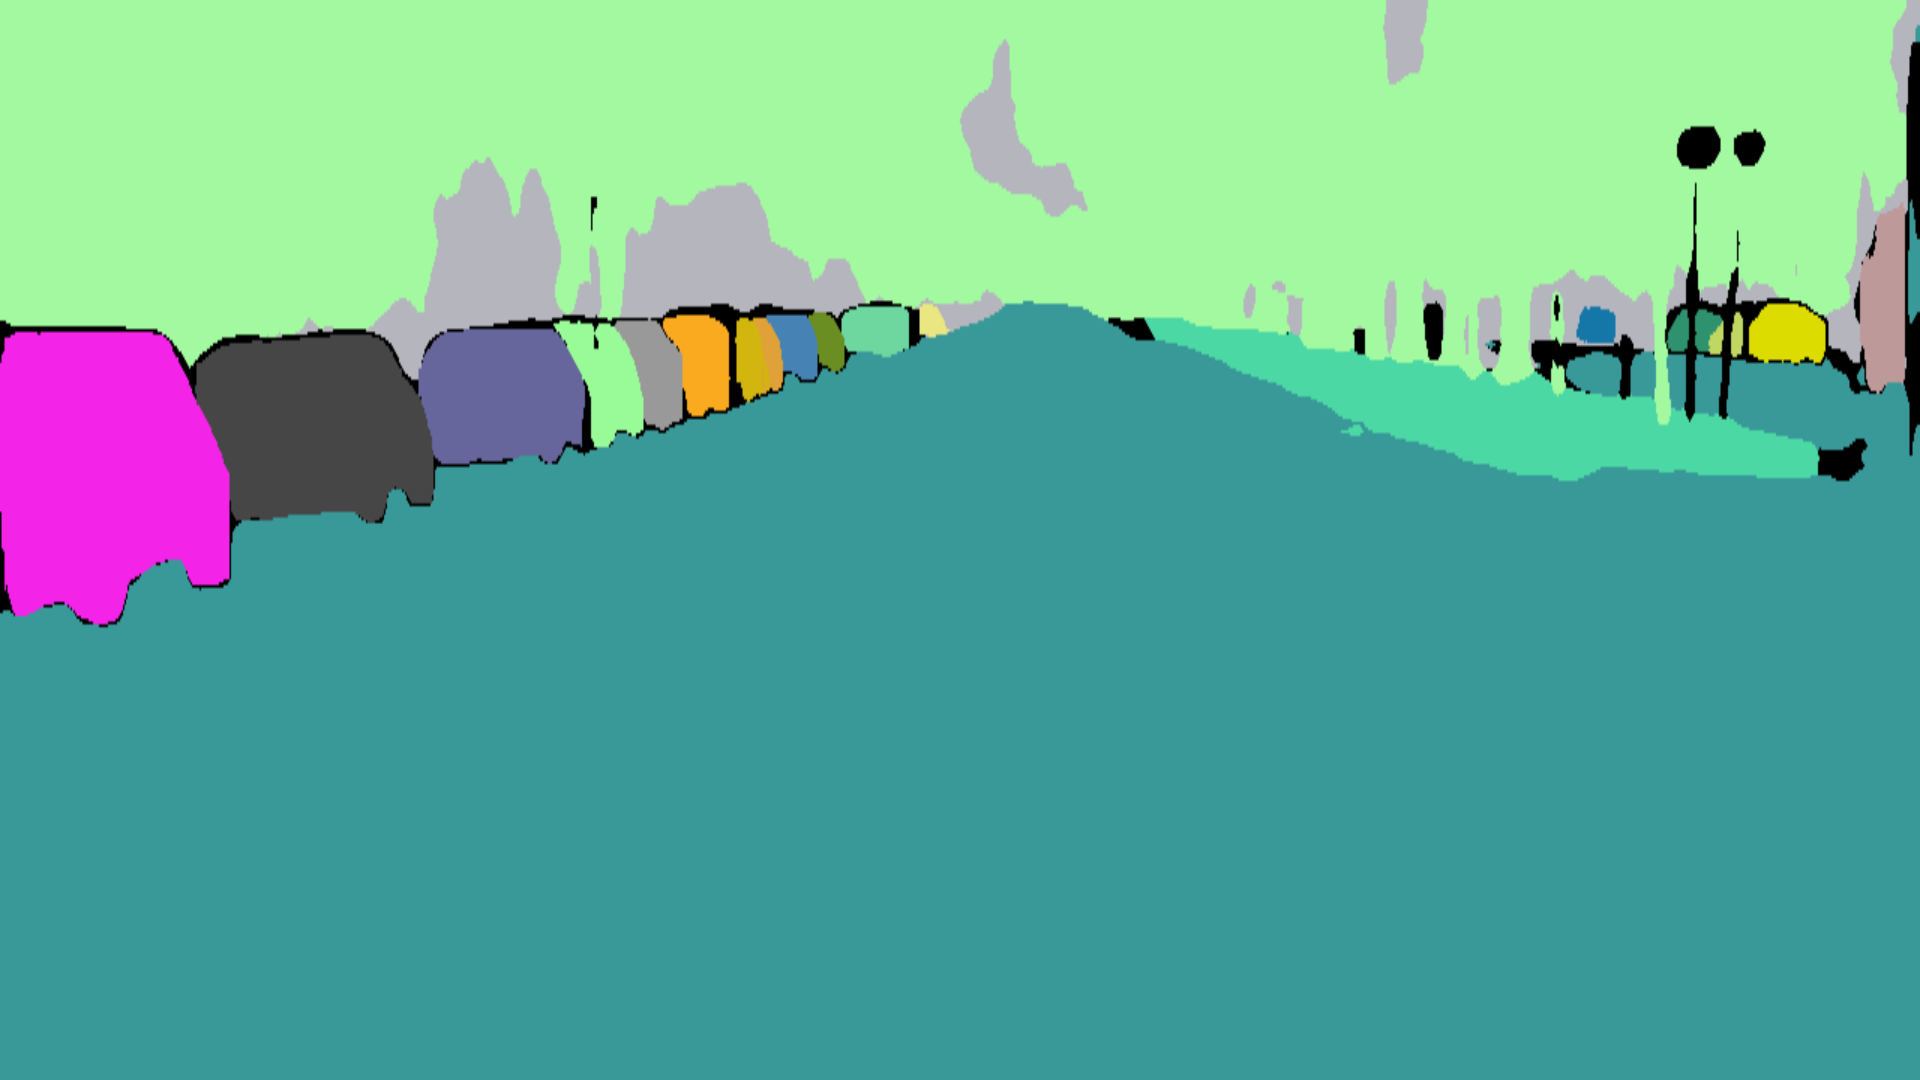
\includegraphics[width=0.6\textwidth]{figures/resultado_obtido.png}
    \legend{Fonte: Criação própria}
	\label{fig:resultado_obtido}
\end{figure}

\subsection{Selecionar contorno}

Para representar a seleção do contorno utilizou-se uma técnica chamada de imagem binária, segundo \citeonline{Embarcados} consiste em isolar um objeto da imagem. Pode-se ser utilizada como uma máscara para auxiliar o processamento do  mapa no contorno desejado \cite{Aznag2020}.

Utilizou-se duas maneiras para selecionar o contorno, sendo elas: selecionar por cor e selecionar por preenchimento de inundação. Selecionar por cor segundo \citeonline{OpenCVInRange} consiste em isolar tudo na imagem com aquela cor, já selecionar por preenchimento de inundação segundo \citeonline{OpenCVFloodFill} consiste em um algoritmo de expansão comparando com uma faixa delimitada de cores. Ambos tem-se como saída uma imagem binária, este pode também ser usado papra selecionar a foto com desenho diretamente.

\subsubsubsection*{Tratamento da imagem binária}

Existem duas forma de tratar a imagem binária.

A primeira, não utilizada pois causa distorção segue após a saída dos algoritmos de seleção, o objeto selecionado é detectado e centralizado em uma nova imagem, depois recortamos e redimensionamos a partir do centro de forma que fique quadrada. Todos os passos são observáveis na \cref{fig:saidas_selecao} \cite{Embarcados}.

\begin{figure}[!ht]
	\centering
    \caption{Passos da seleção da saída da inteligência  artificial.}
	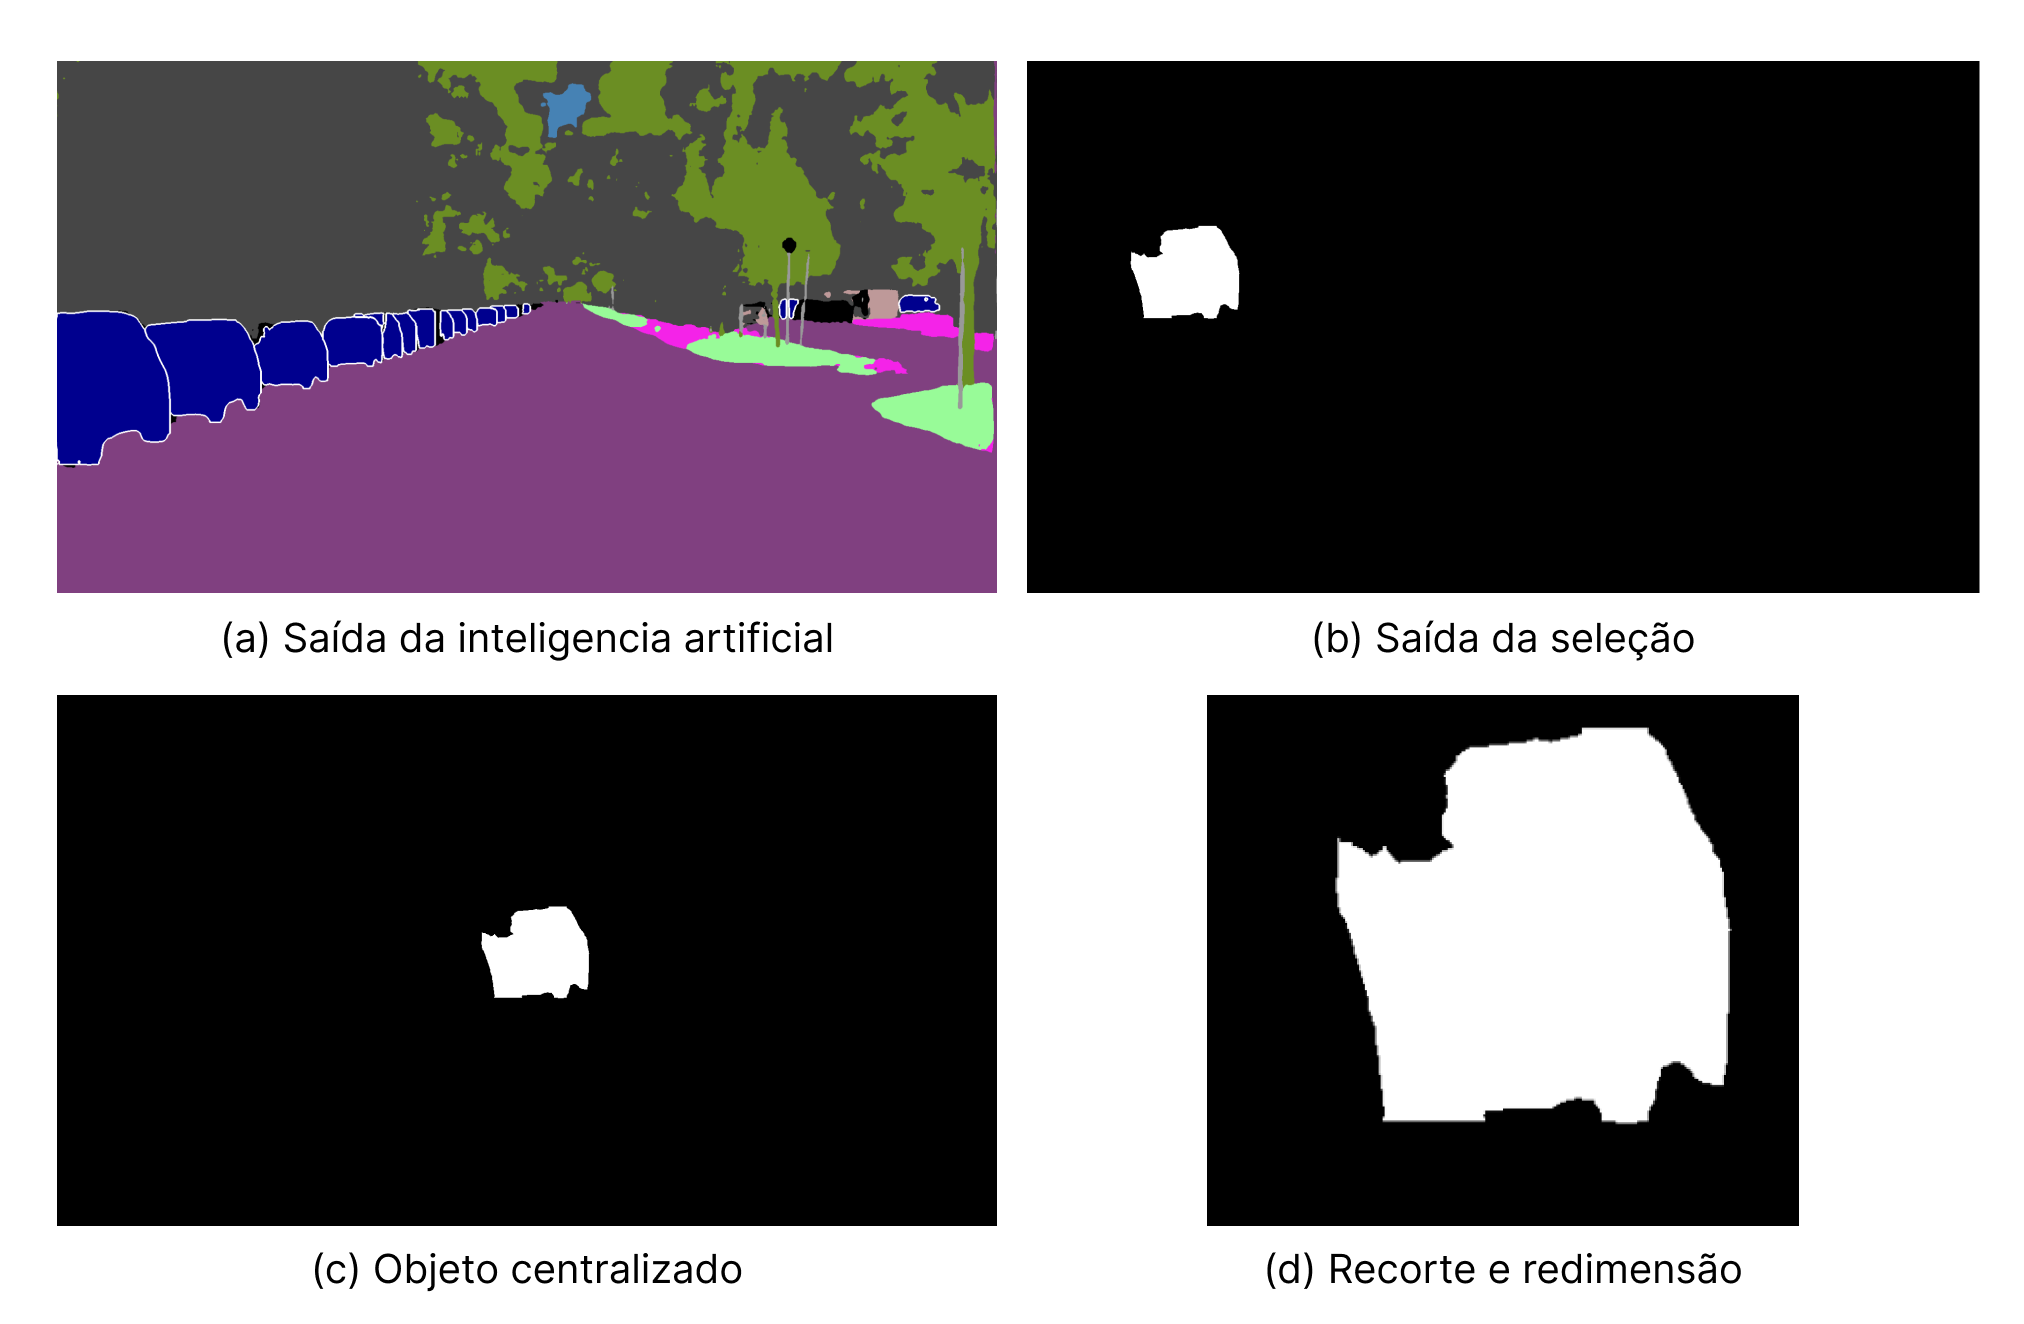
\includegraphics[width=1.0\textwidth]{figures/saidas_selecao.png}
    \legend{Fonte: \space Autoria própria}
	\label{fig:saidas_selecao}
\end{figure}

Já A segunda e mais performática para fazer isso, inclusive melhorando os resultados devido ao redimensionamento e a borda não chegarem a um bom cenário, usa um método para localizar o objeto na imagem binária e corta a imagem com as coordenadas e dimensões oferecidas. Após isso é acrescentado uma borda na altura ou largura com a folga entre as duas, tornando assim a imagem quadricular, depois é redimensionado para manter um padrão e acrescentado mais uma vez uma borda para representar o mar. É possível observar na \cref{fig:saidas_selecao_perf} que o objeto não foi distorcido como na método anterior e manteve-se centralizada na imagem final \cite{Embarcados}.

\begin{figure}[!ht]
	\centering
    \caption{Passos da seleção da saída da inteligência  artificial mais performático.}
	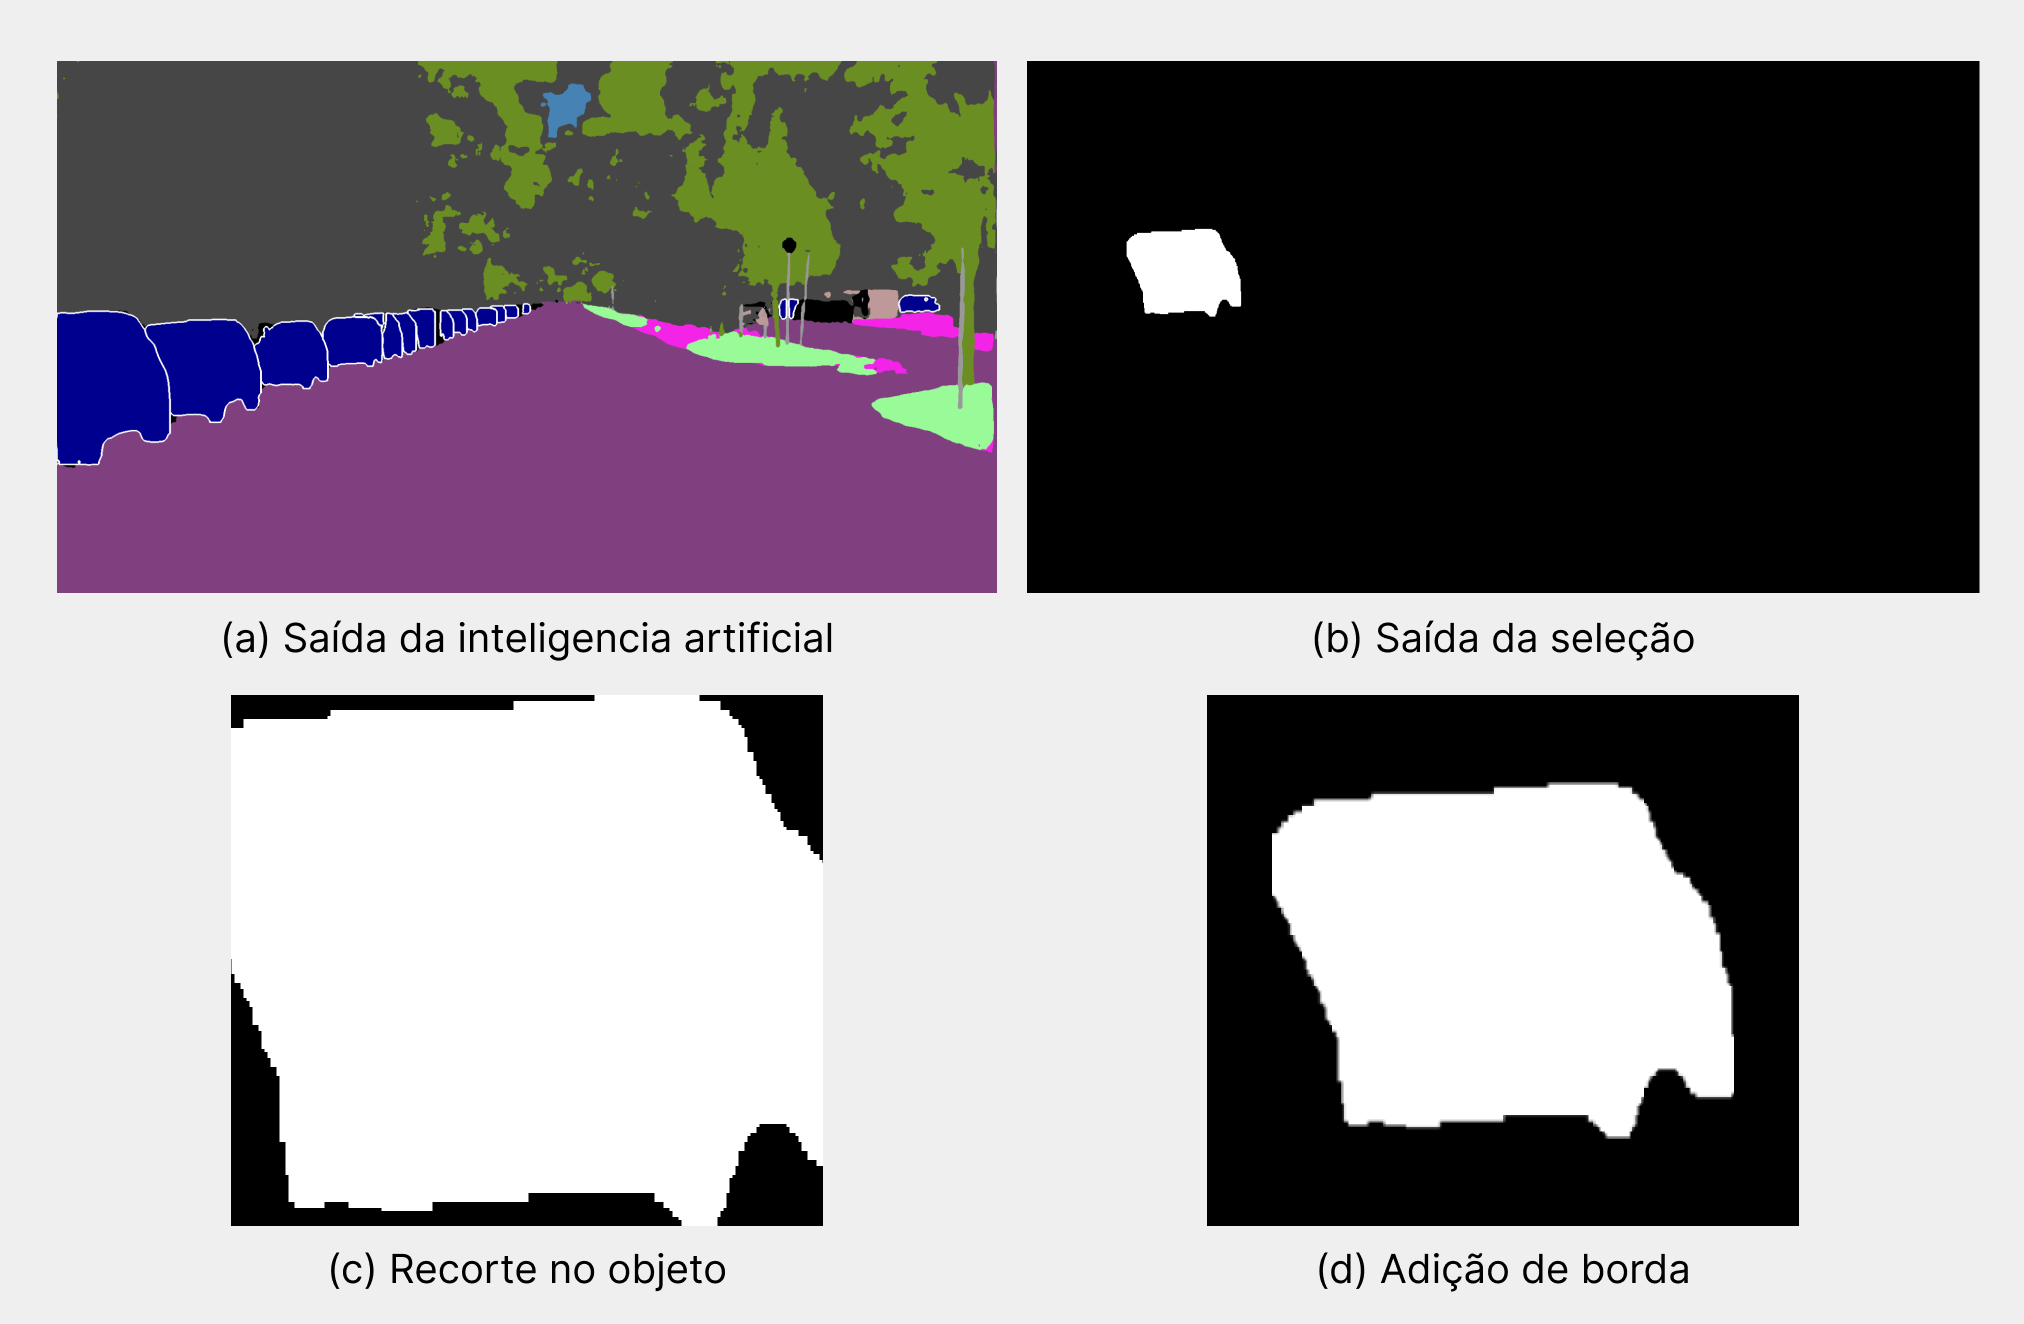
\includegraphics[width=1.0\textwidth]{figures/saidas_selecao_2.png}
    \legend{Fonte: \space Autoria própria}
	\label{fig:saidas_selecao_perf}
\end{figure}

\subsection{Geração procedural do mapa}

Usou-se como base para a geração procedural do mapa o artigo de \citeonline{amitp2010} com uma implementação feita em Python por \citeonline{polygonal-map-generation}.

\subsubsection{Ilha gerada no contorno}

Para gerar o mapa da ilha é preciso gerar um diagrama de Voronoi. No diagrama primeiro é definido os pontos de quantidade preestabelecida e de localização pseudo-aleatória, esses pontos serão os centroides dos polígonos. Os vértices dos polígonos são gerados a partir da intersecção entre retas perpendiculares aos pontos médios entre os nós vizinhos, esses pontos vizinhos são encontrados a partir de uma circunferência no ponto e se existir algum ponto é marcado como vizinho e esse local é chamado de região como descrito na \cref{eq:voronoi_regiao}, logo é criado outro grafo com esses pontos. A definição dos vértices é ilustrada na \cref{fig:explicacao_vertice}, sendo os pontos vermelhos os centroides que são ligados por linhas pretas para gerar pontos médios, representados por pontos amarelos para traçar uma reta perpendicular, depois é calculado a intersecção representado pelo ponto azul que se torna o vértice, e a cor rosa representa a aresta do polígono \cite{amitp2010,rodrigues_diagrama_2019}.

\begin{figure}[!ht]
	\centering
    \caption{Ilustração do processo de criação do polígono.}
	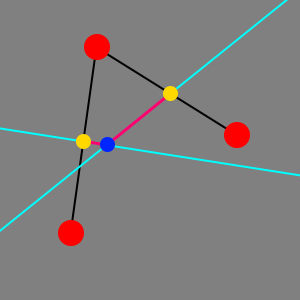
\includegraphics[width=0.6\textwidth]{figures/explicacao_vertice.png}
    \legend{Fonte: Autoria própria}
	\label{fig:explicacao_vertice}
\end{figure}

A \cref{fig:diagrama_voronoi_pontos} ilustra o modelo do diagrama de Voronoi do algoritmo, sendo os pontos vermelhos os centroides que são ligados por linhas pretas, os pontos azuis são os vértices que se ligam com linha branca para tornar as arestas formando assim o polígono.

\begin{figure}[!ht]
	\centering
    \caption{Ilustração do diagrama de Voronoi.}
	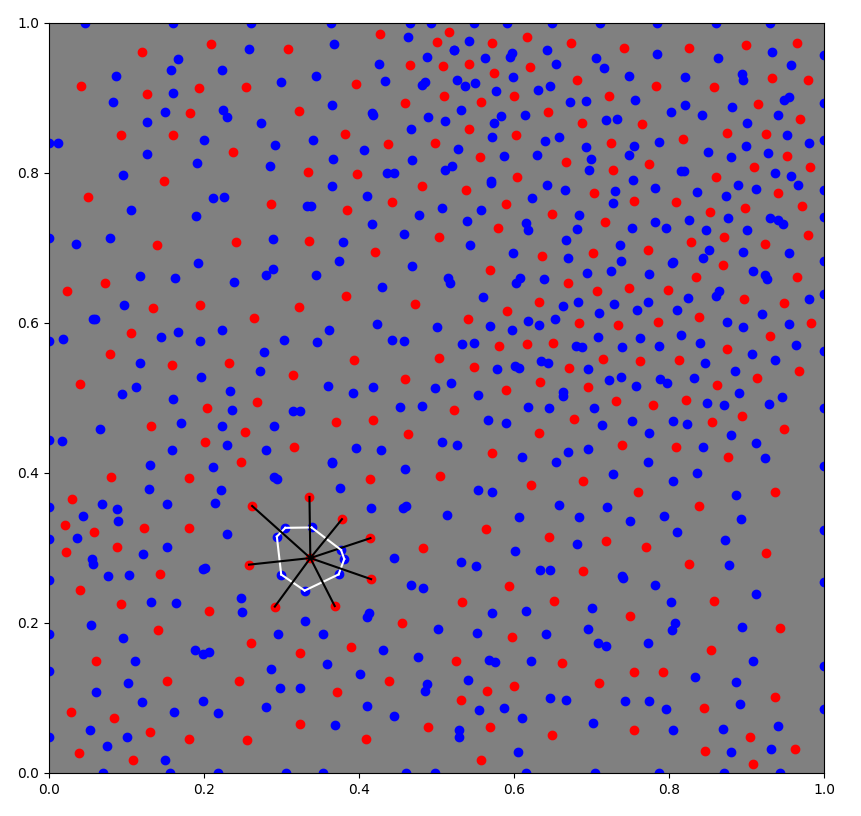
\includegraphics[width=0.6\textwidth]{figures/diagrama_voronoi_pontos.png}
    \legend{Fonte: Autoria própria}
	\label{fig:diagrama_voronoi_pontos}
\end{figure}

Cada polígono criado será nomeado de região e basta definir o tipo do terreno, elevação e umidade. Na lógica, marca-se todos os polígonos com o terreno de tipo oceano. Existem duas formas de selecionar o contorno da image.

A primeira, mais lenta pois necessita verificar todos o pixeis da imagem, percorre-se todos os pontos da imagem de entrada e verifica-se se cada pixel que está contido no objeto da imagem binária encontra-se nos polígonos gerados, se for encontrado adiciona-se o polígono em uma lista de marcação \cite{OpenCV}.

E a segunda, mais performática, pois se utiliza as bibliotecas do OpenCV, faz-se um iteração na lista de polígonos e para cada um é criado uma imagem que é desenhado o polígono da iteração e é feito uma comparação com imagem binaria — o resultado dessa comparação é uma imagem com os pixeis que existem nas duas imagens(binaria e do polígono) —, verifica-se se existe pixeis branco na imagem resultado, se houver adiciona-se o polígono em uma lista de marcação \cite{OpenCV}.

Para os polígonos dentro da lista de marcação, marca-se o tipo do terreno como tipo terra, e em seguida checa-se em quais polígonos do tipo terra são vizinhos do tipo oceano, se sim, define-se como do tipo litoral, e também assina-se os pontos desses polígonos que encontram-se no polígono do tipo oceano \cite{amitp2010,Embarcados}.

Para se calcular a elevação dos polígonos primeiramente é calculado a elevação das arestas de todos os polígonos, isso é feito a partir de uma busca em profundidade que possui o inicio em todas as arestas que tocam a borda do gráfico. A toda nova iteração, as arestas que tocam os cantos são atribuídas com o valor 0, e assim defini-se uma evolução da altura conforme chega-se ao centro do mapa.
Após isso é feito o calculo de redistribuição de elevação, que com base na elevação calculada anteriormente é feito uma lista ordenadas pela elevação, começando da menor para a maior. Cada item da lista é enumerado a partir de um índice i e com essa enumeração é calculado usando a \cref{eq:total_indexes}. Após isso é calculado a \cref{eq:vertex_elevation} sendo X a elevação do vértice.
E por final para calcular a elevação do polígino é feito a média dos vértices que pertencem ao polígonos \cite{amitp2010}.

\begin{equation}
	\label{eq:total_indexes}
	Y = i / total de indices
\end{equation}

\begin{equation}
	\label{eq:vertex_elevation}
	X = sqrt(fator) - sqrt(sqrt * (1 - Y))
\end{equation}

Para criação dos rios busca-se os vértices do tipo terra e litoral que possuem uma elevação miníma definida, ou se os vértices se localizam próximos de um lago, então armazena-se em uma lista. Seleciona-se de forma pseudoaleatória uma quantidade de vértices e verifica-se se o tipo de terreno dos vizinhos dos vértices e das arestas que foram tocados pelos vértices. Para cada um desses é verificado se o tipo de terrenho é terra ou litoral. Após isso, busca-se em todas as arestas a dona do vértice, ao encontrar é marcado como sendo um rio \cite{amitp2010}.

Na geração de umidade é atribuído um valor para cada vértice que possui uma aresta do tipo rio, ou se é vizinho de um lago, e é colocado esse item em uma fila. Logo em seguida, busca-se em profundidade, em todos os vértices adjacentes dos itens da fila, e é calculado uma nova umidade a partir de uma multiplicação de um fator com o valor da umidade anteriormente atribuída, e verifica-se se os vértices adjacentes possuem uma umidade maior que a nova umidade calculada, se forem é colocado o vértice adjacente na fila e é atribuído o valor da nova umidade. Para terrenos do tipo oceano é atribuído o valor máximo de umidade \cite{amitp2010}.

Por fim, é atribuído o valor da umidade para os polígonos e é redistribuído a umidade a partir de uma lista polígonos com umidades ordenadas, para cada item i executa-se a \cref{eq:umidade} e assim é calculado o valor final da umidade \cite{amitp2010}.

\begin{equation}
	\label{eq:umidade}
	i / tamanho(lista) - 1
\end{equation}


Para assinalar os biomas verifica-se o tipo do terreno, altura e a umidade, cada um desses parâmetros liga-se um determinado bioma. E para atribuição final aplica-se a classificação descrita na \cref{fig:diagrama-whittaker}, porem editou-se o eixo de temperatura para elevação para chegar nos resultados da \cref{tab:biomes}, pois o diagrama de Whittaker não leva em consideração a elevação \cite{amitp2010}.

\begin{sidewaystable}
	\centering
	\caption{Relação entre umidade e elevação para biomas}
	\label{tab:biomes}
	\begin{tabularx}{\textwidth}{|X|X|X|X|X|X|X|}
	\hline
	\textbf{Zona de Elevação} & \multicolumn{6}{c|}{\textbf{Zona de Umidade}} \\
	\cline{2-7}
	 & \textbf{6 (úmido)} & \textbf{5} & \textbf{4} & \textbf{3} & \textbf{2} & \textbf{1 (seco)} \\
	\hline
	\textbf{4 (alto)} & \multicolumn{3}{|c|}{NEVE} & TUNDRA & DESNUDO & ESCALDADO  \\
	\hline
	\textbf{3} & \multicolumn{2}{|c|}{TAIGA} & \multicolumn{2}{|c|}{ARBUSTIVO} & \multicolumn{2}{|c|}{DESERTO TEMPERADO} \\
	\hline
	\textbf{2} & FLORESTA TROPICAL TEMPERADA & \multicolumn{2}{|c|}{FLORESTA DECÍDUA TEMPERADA} & \multicolumn{2}{|c|}{GRAMADO} & DESERTO TEMPERADO  \\
	\hline
	\textbf{1 (baixo)} &  \multicolumn{2}{|c|}{FLORESTA CHUVOSA TROPICAL} & \multicolumn{2}{|c|}{FLORESTA SAZONAL TROPICAL} & GRAMADO & DESERTO SUBTROPICAL  \\
	\hline
	\end{tabularx}
\end{sidewaystable}

Para gerar o mapa de três dimensões é gerado uma imagem denominada de mapa de altura, construído com base nos dados de elevações do grafo. Gera-se uma imagem com tonalidades de cinza sendo o pixel branco com valor 255 o ponto mais alto do mapa e o pixel preto com valor 0 o ponto mais baixo, é possível observar isso na \cref{fig:heightmap} \cite{planetzoo}.

\begin{figure}[!ht]
	\centering
    \caption{Exemplo de mapa de altura.}
	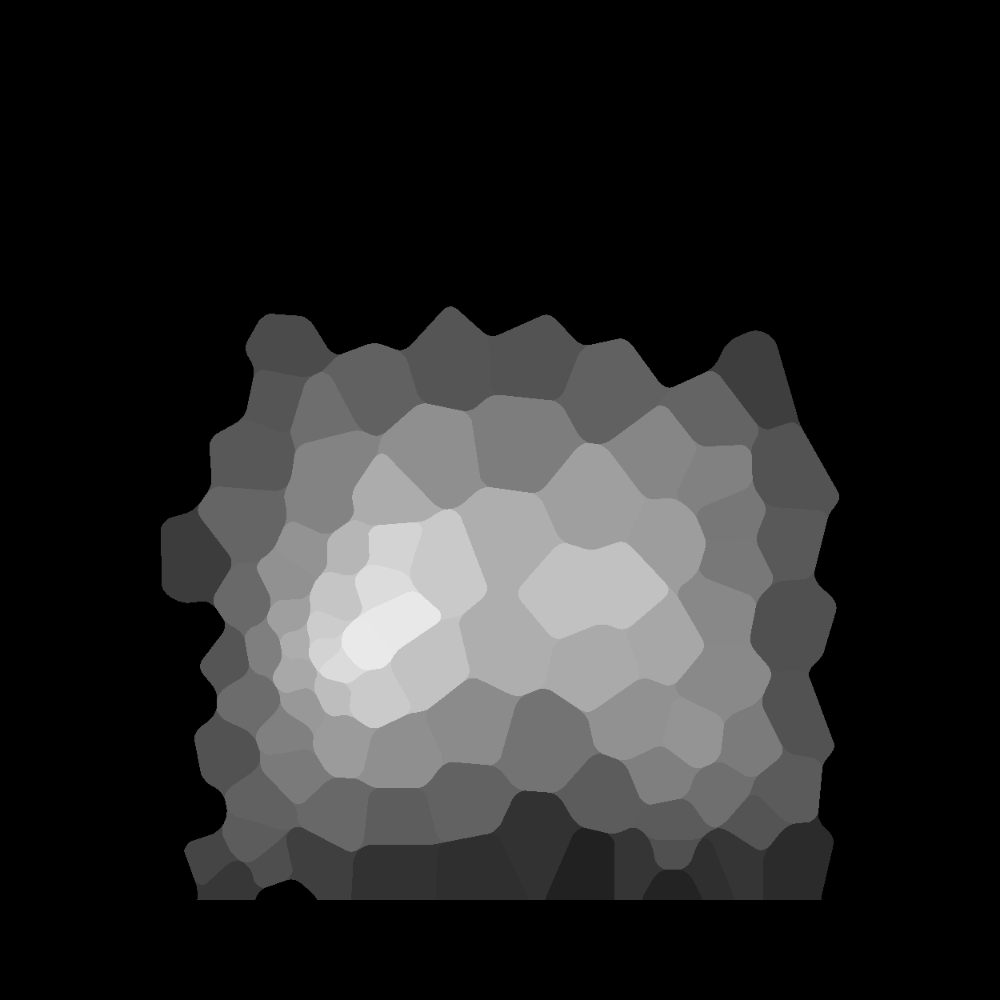
\includegraphics[width=0.6\textwidth]{figures/heightmap_eample.png}
    \legend{Fonte: \space Autoria própria}
	\label{fig:heightmap}
\end{figure}

\subsubsection{Unity - Mapa 3d}

Para demonstrar uma aplicação das imagens utilizou-se o motor gráfico Unity. Criou-se uma automatização entre a geração do mapa e a atualização no projeto Unity. Este processo pode ser dividido em três partes sendo elas o terreno, minimapa em 3D e a jogabilidade \cite{unitywebpage}.

\subsubsubsection{Terreno}
Para atualizar o terreno usou-se primeiramente o pacote \textit{Terrain Tools} que facilita pois é possível usar um mapa de altura em png ou raw para criar um terreno, ao executar cria-se um terreno no qual o pixel mais branco (255) corresponde a altura mais alta \cite{unity-terrain-tools}.

Porém esse processo era manual e a ideia era que fosse automatizado, logo utilizou-se um algoritmo ligado a câmera do personagem que toda vez em que inicia-se a cena atualiza-se o terreno com a nova imagem de mapa 3d em raw. O algoritmo abre a imagem e percorre anotando o relevo proporcional a uma matriz e depois aplica no terreno \cite{unity-terrain-tools}.

Além da funcionalidade de relevo adicionou-se um pacote para alterar a textura de acordo com a altura para diferenciar o oceano da ilha e o bioma de floresta. Utilizou-se o pacote denominado de \textit{Terrain Toolkit 2017}, no script é carregado as texturas e definido alguns parâmetros para atualizar com o terreno \cite{unity-terrain-toolkit}.

\subsubsubsection{Minimapa}
A saída da geração procedural visa dois principais resultados, sendo eles: o mapa de altura para definir o terreno e o mapa 2d que pode ser usado como minimapa \cite{unitywebpage}.

Para usar o mapa 2d como minimapa de forma automatizada foi necessário adicionar nos \textit{scripts} uma conversão de uma imagem em formato PNG para um Sprite (2D e UI) e atualizar nas propriedades do objeto de jogo. Possibilitando a localização de um ícone representando o jogador nesse minimapa por meio da projeção das coordenadas 3D do mundo do jogo em um mapa 2D \cite{unitywebpage}.

\subsubsubsection{Jogabilidade}

Criou-se um personagem com movimentação para andar pelo mapa baseado no vídeo no Youtube de \citeonline{firstPersonMovement}. Adicionando os objetos e o script principal além de criar uma tag de chão para detectar a colisão é possível jogar no mapa andando em todas as direções e pulando.

\subsection{Testes}

Criou-se testes para comparar uma combinação de imagens, podendo conter a imagem de entrada do algoritmo de geração procedural ou alguma saída, mapa de altura ou mapa 2d. Para mensurar a qualidade usou-se como base a técnica descrita por \citeonline{kirillov2019panoptic} chamada de classificação dos conjuntos, na qual cria uma nova imagem em que cada pixel será de algum conjunto dentre quatro: Verdadeiros positivos, Verdadeiros negativos, Falsos positivos e Falsos negativos. A \cref{fig:representacao} apresenta a ilustração da classificação dos conjuntos, sendo a imagem a, a imagem de entrada para geração procedural (saída da seleção), a imagem b, o mapa de altura que é uma das saídas da geração procedural, a imagem c, o filtro binário a partir do mapa de altura, ou seja, apenas os pixeis com cor monocromática zero serão mantidos como preto e qualquer alteração será marcado como branco, a imagem d, é a ilustração dos conjuntos entre a imagem de entrada e o filtro binário do mapa de altura, sendo a cor cinza o união entre cores pretas, a cor branca é a união de cores brancas, a cor verde quando a imagem de entrada tem cor branca porém o filtro binário tem cor preta e por fim a cor vermelha é quando o filtro tem a cor branca porém na imagem de entrada tem a cor preta.

\begin{figure}[!ht]
	\centering
    \caption{Ilustração da classificação de conjuntos}
	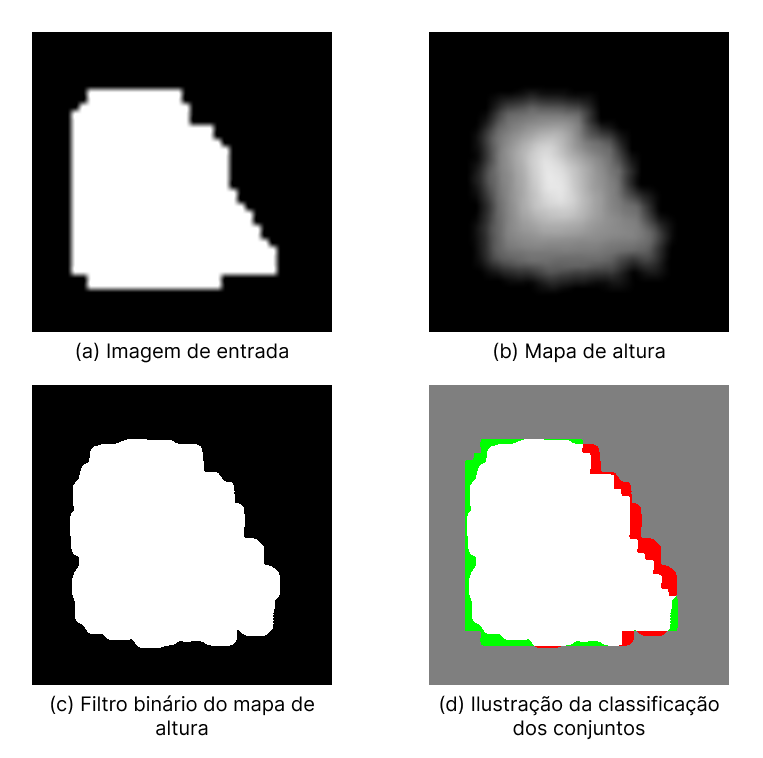
\includegraphics[width=0.8\textwidth]{figures/representacao_classificacao.png}
    \legend{Fonte: \space Autoria própria}
	\label{fig:representacao}
\end{figure}

Depois foi contabilizou-se esses pixeis com cores diferentes para utilizar em diversas métricas baseadas na classificação dos conjuntos, sendo elas: F1 Score, Coeficiente de correlação de Matthews, Taxa de descoberta falsa, Taxa de Falso Negativo, Acurácia e União sobre intersecção \cite{Chicco2020, confusion_matrix_calculator, iou_metric_link}.

% A métrica IoU pois esta é a que pior classifica nosso modelo e também facilita a percepção de melhora, metrificando a semelhança obtida do contorno desejado. Portanto quanto maior essa métrica maior a compatibilidade com o contorno inicialmente proposto.

Além dessas métricas, utilizou-se também uma métrica para o desfoque encontrado em uma imagem, aplica-se um filtro para detectar bordas em x e y, calcula o gradiente e resulta o desvio padrão, isso serve para mensurar a harmonia do mapa de alturas. Outra métrica utilizada nos testes foi a duração do tempo no código, medida em segundos e apenas contabilizando a parte de geração procedura dos mapas.

Criou-se um teste genérico para reutilizar em diversos testes e facilitar a reprodução caso haja mudanças. É definido na chamada do teste as imagens e métricas, com isso é possível definir todas combinações possíveis. Para cada combinação será executado 5 imagens de entrada pré-definidas e em cada imagem irá percorrer um laço baseado em alguma variável de geração procedural sendo elas: tamanho do filtro de desfoque, quantidade de pontos ou tamanho da borda no mapa 2d. Em cada iteração da variável, será executado três vezes.

Em cada iteração de todos esses laços aninhados será gerado proceduralmente algum mapa ou os dois, processado as métricas e armazenado, após isso será calculado a média das métricas e criado uma tabela em \LaTeX como resultado.

\subsection{Pós processamento}
Analisando-se o resultado gerado no Unity do mapa 3d na \cref{fig:Unity_init} percebe-se que não existe uma harmonia entre os biomas e por isso gerou-se uma solução aplicando um desfoque na imagem de mapa de altura para suavizar a mudança de biomas.

\begin{figure}[!ht]
	\centering
    \caption{Resultado no Unity sem usar filtro de desfoque no mapa de altura.}
	\includegraphics[width=0.8\textwidth]{figures/Unity_entry.png}
    \legend{Fonte: \space Autoria própria}
	\label{fig:Unity_init}
\end{figure}

Aplicando um filtro — ou kernel — de desfoque com tamanho 100x100, obteve-se o resultado ilustrado na \cref{fig:Unity_blur}. Porém, ao analisar a \cref{tab:blur_error_input_output_3d} observa-se que as métricas pioraram. Isso permite concluir que o desfoque comprometeu a qualidade da equivalência dos contornos, exacerbando um problema de escala. Este problema fica evidente pelo fato de que apenas o erro no mapa de altura foi detectado. Na \cref{fig:comparando_blur} observa-se uma representação visual da classificação dos conjuntos definido em \citeonline{kirillov2019panoptic}, sendo a imagem a, o resultado da comparação entre a imagem de entrada e a saída do mapa de altura sem desfoque, sendo o vermelho o erro encontrado no mapa de altura (está branco no mapa de altura mas preto no de entrada), e a imagem b, sendo o mesmo caso porém aplicando o filtro de desfoque.

\begin{figure}[!ht]
	\centering
    \caption{Resultado no Unity usando filtro de desfoque no mapa de altura.}
	\includegraphics[width=0.8\textwidth]{figures/Unity_blur.png}
    \legend{Fonte: \space Autoria própria}
	\label{fig:Unity_blur}
\end{figure}

\begin{table}[h]
            \centering
            \caption{Resultados dos testes de contorno}
            \label{tab:resultados-contorno}
            \begin{tabular}{|c|c|c|}
                \hline
                                Tamanho filtro & IoU & Blur \\
                \hline
                0 & 0.7385 & 53.49246\\
        100 & 0.60484 & 9.75581\\
                \hline
            \end{tabular}
        \end{table}




\begin{figure}[!ht]
	\centering
    \caption{Ilustração da classificação de conjuntos entre a imagem de entrada e o mapa de altura}
	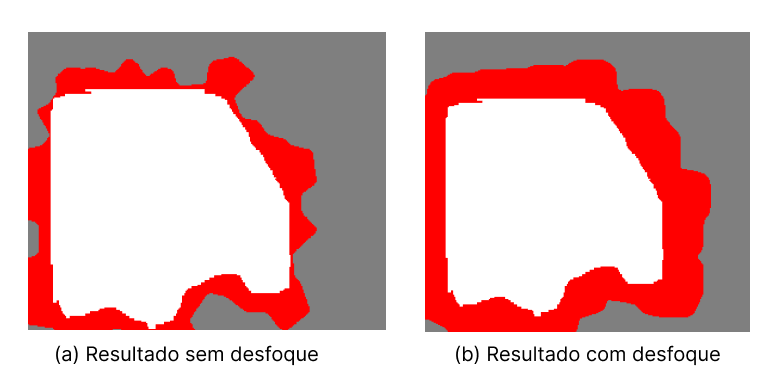
\includegraphics[width=0.8\textwidth]{figures/comparacao_blur.png}
    \legend{Fonte: \space Autoria própria}
	\label{fig:comparando_blur}
\end{figure}

Logo para tratar esse problema adotou-se uma solução baseada em redimensionar a imagem e adicionar uma borda para que diminui-se assim o tamanho do mapa de altura. Portanto foi redimensionado uma imagem 1000x1000 para 800x800, reduzindo em 20\% e depois adicionado uma borda de cor preta em todos os lados de tamanho 100, logo retorna ao tamanho original. E para encontrar o melhor tamanho do filtro de desfoque para essas condições executou-se os testes alterando o tamanho do filtro apos a aplicação da técnica de diminuir o tamanho do mapa. Os resultados referentes aos testes encontram-se na \cref{tab:blur_solution_input_output_3d}. Para selecionar o melhor resultado definiu-se a quesito de ter a menor métrica de desfoque — que significa ter mais desfoque na imagem — e com a métrica IoU que varie no máximo 1\% da métrica sem o filtro de desfoque. Logo seleciona-se o resultado de filtro de tamanho 80 pois a métrica IoU tem 79\% assim como o tamanho de filtro 0. Percebe-se também que com a diminuição da borda resultou no compartilhamento entre os erros da imagem de entrada com o mapa de altura.

\begin{table}[h]
    \centering
    \caption{Resultados dos testes entre imagem de entrada e output3d}
    \label{tab:blur_solution_input_output_3d}
    \begin{tabular}{|c|c|c|c|c|}
        \hline
        Tamanho filtro & Desfoque & IoU & FDR & FNR \\
        \hline
        100 & 11.35778 & 0.76178 & 0.22752 & 0.01707\\
        90 & 11.88265 & 0.76887 & 0.2162 & 0.02281\\
        80 & 12.37601 & 0.79299 & 0.18761 & 0.02824\\
        70 & 13.59314 & 0.79101 & 0.18298 & 0.03676\\
        60 & 14.75522 & 0.80283 & 0.16196 & 0.04787\\
        50 & 16.29726 & 0.81851 & 0.13458 & 0.06073\\
        40 & 18.35148 & 0.81608 & 0.12325 & 0.07635\\
        30 & 21.52558 & 0.81866 & 0.10467 & 0.0935\\
        20 & 27.79682 & 0.8183 & 0.08627 & 0.11246\\
        10 & 38.13084 & 0.80744 & 0.07181 & 0.13757\\
        0 & 48.89338 & 0.79895 & 0.05978 & 0.15749\\
        \hline
    \end{tabular}
\end{table}




Após melhorar o resultado do mapa de entrada é necessário ajustar o mapa 2d visto que esse deve ser bem parecido com o mapa de altura, parar informar por exemplo a localização exata do personagem em jogo com visualização do mapa inteiro. Observa-se na \cref{tab:border_2d_solution_output_2d_output_3d} os resultados obtidos dos testes com o tamanho da borda adicionada ao mapa 2d e o maior valor de IoU obtido foi 60.

\begin{table}[h]
    \centering
    \caption{Resultados dos testes entre mapa 2d e mapa de altura}
    \label{tab:border_2d_solution_output_2d_output_3d}
    \begin{tabular}{|c|c|c|c|}
        \hline
        Tamanho borda & IoU & FDR & FNR \\
        \hline
        0 & 0.82075 & 0.02435 & 0.16192\\
        10 & 0.84148 & 0.02679 & 0.13833\\
        20 & 0.86438 & 0.03616 & 0.10622\\
        30 & 0.87938 & 0.04263 & 0.0846\\
        40 & 0.89456 & 0.05307 & 0.0578\\
        50 & 0.90031 & 0.06612 & 0.03827\\
        60 & 0.90771 & 0.07929 & 0.0152\\
        70 & 0.89229 & 0.10441 & 0.00408\\
        80 & 0.86867 & 0.13132 & 1e-05\\
        90 & 0.84037 & 0.15963 & 0.0\\
        100 & 0.81396 & 0.18604 & 0.0\\
        \hline
    \end{tabular}
\end{table}




\subsection{Interface gráfica}

Utilizou-se a biblioteca PyQt5 para criar uma interface gráfica na qual o usuário poderá interagir e criar um mapa a partir da seleção do contorno detectado pelo modelo de IA.

Esse módulo é responsável para conectar todas as partes e obter o mapa. Portanto é necessário abrir uma imagem do diretório local, carregar e disparar a execução do processo de segmentação de imagem. Após o resultado da IA, permitir a seleção do contorno,  criar uma imagem binária a partir do contorno e envia-lá como argumento na geração procedural de mapas.

Além disso para promover a usabilidade utilizou-se um \textit{loading} específico para PyQt5 e para isso teve-se que usar threads, criando classes para rodar as tarefas de forma separada e síncrona.